% 若编译失败,且生成 .synctex(busy) 辅助文件,可能有两个原因:
% 1. 需要插入的图片不存在:Ctrl + F 搜索 'figure' 将这些代码注释/删除掉即可
% 2. 路径/文件名含中文或空格:更改路径/文件名即可

% 设定文章编码类型,正文字号为五号,若需小四将 5 改为 -4 即可
\documentclass[zihao=5,UTF8]{report}		


% 自定义宏定义
\def\N{\mathbb{N}}
\def\F{\mathbb{F}}
\def\Z{\mathbb{Z}}
\def\Q{\mathbb{Q}}
\def\R{\mathbb{R}}
\def\C{\mathbb{C}}
\def\T{\mathbb{T}}
\def\S{\mathbb{S}}
\def\A{\mathbb{A}}
\def\I{\mathscr{I}}
\def\d{\mathrm{d}}
\def\p{\partial}


% 导入基本宏包
\usepackage[UTF8]{ctex}     % 设置文档为中文语言
\usepackage[colorlinks, linkcolor=blue, anchorcolor=blue, citecolor=blue, urlcolor=blue]{hyperref}  % 宏包:自动生成超链接 (此宏包与标题中的数学环境冲突)
% \usepackage{docmute}    % 宏包:子文件导入时自动去除导言区,用于主/子文件的写作方式,\include{./51单片机笔记}即可。注:启用此宏包会导致.tex文件capacity受限。
\usepackage{amsmath}    % 宏包:数学公式
\usepackage{mathrsfs}   % 宏包:提供更多数学符号
\usepackage{amssymb}    % 宏包:提供更多数学符号
\usepackage{pifont}     % 宏包:提供了特殊符号和字体
\usepackage{extarrows}  % 宏包:更多箭头符号


% 文章页面margin设置
\usepackage[a4paper]{geometry}
    \geometry{top=1in}
    \geometry{bottom=1in}
    \geometry{left=0.75in}
    \geometry{right=0.75in}   % 设置上下左右页边距
    \geometry{marginparwidth=1.75cm}    % 设置边注距离(注释、标记等)


\usepackage{amsthm} % 宏包:数学环境配置
% theorem环境自定义
    \newtheoremstyle{MyTheoremStyle}% <name>
        {11pt}% <space above>
        {11pt}% <space below>
        {}% <body font> 使用默认正文字体
        {}% <indent amount>
        {\bfseries}% <theorem head font> 设置标题项为加粗
        {:\\ }% <punctuation after theorem head>
        {.5em}% <space after theorem head>
        {\textbf{#1}\thmnumber{#2}\ \ (\,\textbf{#3}\,)}% 设置标题内容顺序
    \theoremstyle{MyTheoremStyle} % 应用自定义的定理样式
    \newtheorem{theorem}{Theorem.\,}
% definition 环境自定义
    \newtheoremstyle{MySubsubsectionStyle}% <name>
        {11pt}% <space above>
        {11pt}% <space below>
        {}% <body font> 使用默认正文字体
        {}% <indent amount>
        {\bfseries}% <theorem head font> 设置标题项为加粗
        {:\\ \indent}% <punctuation after theorem head>
        {0pt}% <space after theorem head>
        {\textbf{#3}}% 设置标题内容顺序
    \theoremstyle{MySubsubsectionStyle} % 应用自定义的定理样式
    \newtheorem{definition}{}

%宏包:有色文本框及其设置
\usepackage[dvipsnames,svgnames]{xcolor}    %设置插入的文本框颜色
\usepackage[strict]{changepage}     % 提供一个 adjustwidth 环境
\usepackage{framed}     % 实现方框效果
    \definecolor{graybox_color}{rgb}{0.95,0.95,0.96} % 文本框颜色。修改此行中的 rgb 数值即可改变方框纹颜色,具体颜色的rgb数值可以在网站https://colordrop.io/ 中获得。(截止目前的尝试还没有成功过,感觉单位不一样)(找到喜欢的颜色,点击下方的小眼睛,找到rgb值,复制修改即可)
    \newenvironment{graybox}{%
    \def\FrameCommand{%
    \hspace{1pt}%
    {\color{gray}\small \vrule width 2pt}%
    {\color{graybox_color}\vrule width 4pt}%
    \colorbox{graybox_color}%
    }%
    \MakeFramed{\advance\hsize-\width\FrameRestore}%
    \noindent\hspace{-4.55pt}% disable indenting first paragraph
    \begin{adjustwidth}{}{7pt}%
    \vspace{2pt}\vspace{2pt}%
    }
    {%
    \vspace{2pt}\end{adjustwidth}\endMakeFramed%
    }

% chapter标题自定义设置
\usepackage{titlesec}   
    \titleformat{\chapter}[hang]{\normalfont\huge\bfseries\centering}{第\,\thechapter\,章}{20pt}{}
    \titlespacing*{\chapter}{0pt}{-20pt}{20pt} % 控制上方空白的大小
    % section标题自定义设置 
    \titleformat{\section}[hang]{\normalfont\Large\bfseries}{§\,\thesection\,}{8pt}{}
    % subsubsection标题自定义设置
    %\titleformat{\subsubsection}[hang]{\normalfont\bfseries}{}{8pt}{}

% 外源代码插入设置
\usepackage{matlab-prettifier}
    \lstset{
        style=Matlab-editor,  % 继承matlab代码颜色等
    }
\usepackage[most]{tcolorbox} % 引入tcolorbox包 
\usepackage{listings} % 引入listings包
    \tcbuselibrary{listings, skins, breakable}
    \lstdefinestyle{matlabstyle}{
        language=Matlab,
        basicstyle=\small,
        breakatwhitespace=false,
        breaklines=true,
        captionpos=b,
        keepspaces=true,
        numbers=left,
        numbersep=15pt,
        showspaces=false,
        showstringspaces=false,
        showtabs=false,
        tabsize=2
    }
    \newtcblisting{matlablisting}{
        arc=0pt,
        top=0pt,
        bottom=0pt,
        left=1mm,
        listing only,
        listing style=matlabstyle,
        breakable,
        colback=white   % 选一个合适的颜色
    }

% table设置
\usepackage{booktabs}   % 宏包:三线表
\usepackage{tabularray} % 宏包:表格排版
\usepackage{longtable}  % 宏包:长表格

% figure设置
\usepackage{graphicx}  % 支持 jpg, png, eps, pdf 图片 
\usepackage{svg}       % 支持 svg 图片
    \svgsetup{
        % 指向 inkscape.exe 的路径
        inkscapeexe = D:/aa_my_apps_main/Inkscape/bin/inkscape.exe, 
        % 一定程度上修复导入后图片文字溢出几何图形的问题
        inkscapelatex = false                 
    }

\usepackage{amssymb}   %  

% 图表进阶设置
\usepackage{caption}    % 图注、表注
    \captionsetup[figure]{name=图}  
    \captionsetup[table]{name=表}
    \captionsetup{labelfont=bf, font=small}
\usepackage{float}     % 图表位置浮动设置 

% 文章默认字体设置
\usepackage{fontspec}   % 宏包:字体设置
    \setmainfont{SimSun}    % 设置中文字体为宋体字体
    \setmainfont{Times New Roman} % 设置英文字体为Times New Roman

% 参考文献引用设置
    \bibliographystyle{unsrt}   % 设置参考文献引用格式为unsrt
    \newcommand{\upcite}[1]{\textsuperscript{\cite{#1}}}     % 自定义上角标式引用

% 文章序言设置
    \newcommand{\cnabstractname}{序言}
    \newenvironment{cnabstract}{%
        \par\Large
        \noindent\mbox{}\hfill{\bfseries \cnabstractname}\hfill\mbox{}\par
        \vskip 2.5ex
        }{\par\vskip 2.5ex}

% 页眉页脚设置
\usepackage{fancyhdr}   %宏包:页眉页脚设置
    \pagestyle{fancy}
    \fancyhf{}
    \cfoot{\thepage}
    \renewcommand\headrulewidth{1pt}
    \renewcommand\footrulewidth{0pt}
    \chead{here is the header,这里是页眉}    


%文档信息设置
\title{这里是标题\\The Title of the Report}
\author{丁毅\\ \footnotesize 中国科学院大学,北京 100049\\ Yi Ding \\ \footnotesize University of Chinese Academy of Sciences, Beijing 100049, China}
\date{\footnotesize 2024.8 -- 2025.1}

% 开始编辑文章

\begin{document}
\maketitle
\newpage

\addcontentsline{toc}{chapter}{序言} % 手动添加为目录
\thispagestyle{fancy}   % 显示页码、页眉等
\begin{cnabstract}
\normalsize 本文为笔者本科时的某课程笔记。用灰色字体或灰色方框等表示对主干内容的补充、对晦涩概念的理解、定理的具体证明过程等,采用红色字体对重点部分进行强调,同时适当配有插图。这样的颜色和结构安排既突出了知识的主要框架,也保持了笔记的深度和广度,并且不会因为颜色过多而导致难以锁定文本内容,乃是尝试了多种安排后挑选出的最佳方案。如果读者有更佳的颜色和排版方案,可以将建议发送到笔者邮箱 dingyi233@mails.ucas.ac.cn,在此感谢。\par
由于个人学识浅陋,认识有限,书中难免有不妥甚至错误之处,望读者不吝指正,在此感谢。

\end{cnabstract}
\pagenumbering{Roman} % 页码为大写罗马数字

\tableofcontents    % 目录页  
\thispagestyle{fancy}   % 显示页码、页眉等         

\newpage
\pagenumbering{arabic} 


\chapter{基础知识}\thispagestyle{fancy} 
\section{第一章第一节}


\begin{definition}[向后加权隐式格式]

将向前差分与向后差分加权组合起来,得到:

\begin{equation}\label{公式5}
    \frac{u_{j}^{k}-u_{j}^{k-1}}{h_t}=a\theta\frac{u_{j+1}^{k}-2u_{j}^{k}+u_{j-1}^{k}}{h_x^2}+a(1-\theta)\frac{u_{j+1}^{k-1}-2u_{j}^{k-1}+u_{j-1}^{k-1}}{h_x^2}
\end{equation}

其中 $\theta \in [0, 1]$ 为权重,其截断误差 $R = a\left(\frac{1}{2}-\theta\right)h_t\left[\frac{\partial^{3}u}{\partial x^{2}\partial t}\right]_{j}^{k}+O(h_t^{2}+h_x^2)$,因此当 $\theta = \frac{1}{2}$ 时,方程具有 $O(h_t^{2}+h_x^2)$ 精度,称为 Crank-Nicolson 格式(CN 格式)。


公式 \ref{公式5} 的增长因子及稳定性条件为:

\begin{equation}
    G(h_t,\sigma)=\frac{1-4(1-\theta)ar\sin^2\frac{\sigma h}2}{1+4\theta ar\sin^2\frac{\sigma h}2}, \ \ 
    \begin{cases}
        r\leqslant\frac{1}{2a(1-2\theta)}, & \theta \in [0, \frac{1}{2}) \\ 
        \text{无条件稳定}, & \theta \in [\frac{1}{2}, 1] \\ 
    \end{cases}
\end{equation}

\begin{theorem}[这是一个定理]\label{这是一个定理}
    你好你好你好
\end{theorem}


\begin{graybox}
\textbf{定理 \ref{这是一个定理} 的证明:}\\
你好你好你好
\end{graybox}

\begin{figure}[H]
    \centering
    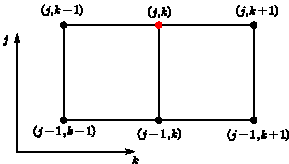
\includegraphics[width=0.5\textwidth]{assets/差分格式示意图.pdf}
    \caption{\textbf{插入pdf图片}}\label{插入pdf图片}
\end{figure}
\end{definition}

\begin{figure}[H]
    \centering
    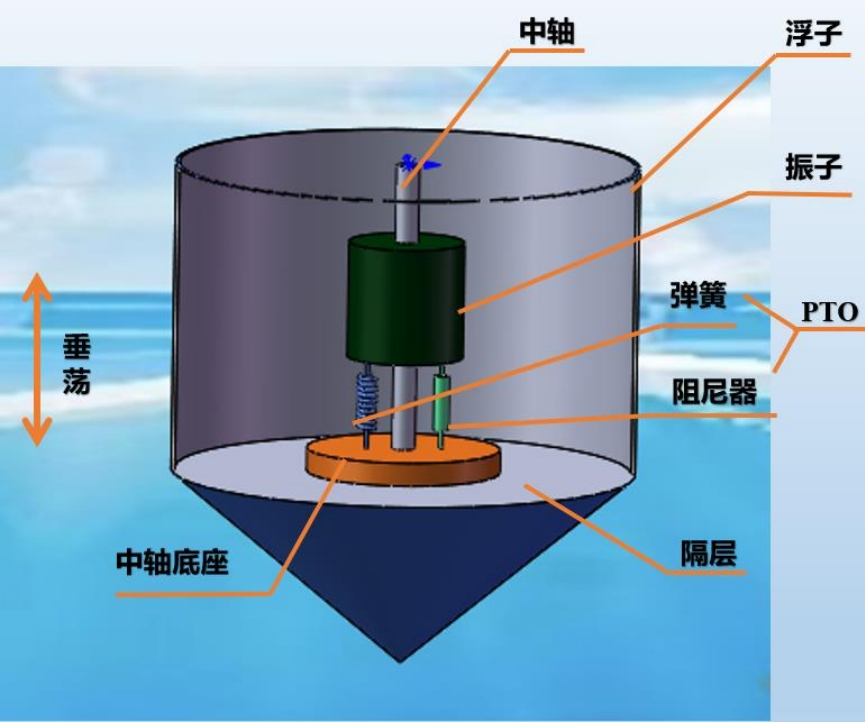
\includegraphics[width=0.5\textwidth]{assets/波浪能装置示意图.jpg}
    \caption{\textbf{插入 jpg}}\label{插入 jpg}
\end{figure}

\begin{figure}[H]
    \centering
    \includesvg[width=0.5\textwidth]{assets/draw.io_test.drawio.svg}
    \caption{\textbf{插入 svg}}\label{插入 svg}
\end{figure}

表格:

\begin{table}[H]
    \centering
    \caption{\textbf{符号含义与约定}}
    \label{tab:waterpump}
    \begin{tabular}{ccccc}
    \toprule
    符号 & 符号含义& 单位\\
    \midrule
    符号1& 含义1& 单位1\\
    符号2& 含义2& 单位2\\
    符号3& 含义3& 单位3\\
    符号4& 含义4& 单位4\\
    \bottomrule
    \end{tabular}
\end{table}

\chapter{这里是第二章}\thispagestyle{fancy} 

\href{https://www.latex-tables.com/}{Latex Table Editor} 示例:

% \usepackage{tabularray}

\begin{longtblr}[caption={\bfseries 示例表格},label=tab:example]{
    hline{1,51} = {-}{0.08em},
    hline{2} = {-}{},
  }
   $x$& hello & $123.456$ \\
   $x$& hello & $123.456$ \\
   $x$& hello & $123.456$ \\
   $x$& hello & $123.456$ \\
   $x$& hello & $123.456$ \\
   $x$& hello & $123.456$ \\
   $x$& hello & $123.456$ \\
   $x$& hello & $123.456$ \\
   $x$& hello & $123.456$ \\
   $x$& hello & $123.456$ \\
   $x$& hello & $123.456$ \\
   $x$& hello & $123.456$ \\
   $x$& hello & $123.456$ \\
   $x$& hello & $123.456$ \\
   $x$& hello & $123.456$ \\
   $x$& hello & $123.456$ \\
   $x$& hello & $123.456$ \\
   $x$& hello & $123.456$ \\
   $x$& hello & $123.456$ \\
   $x$& hello & $123.456$ \\
   $x$& hello & $123.456$ \\
   $x$& hello & $123.456$ \\
   $x$& hello & $123.456$ \\
   $x$& hello & $123.456$ \\
   $x$& hello & $123.456$ \\
   $x$& hello & $123.456$ \\
   $x$& hello & $123.456$ \\
   $x$& hello & $123.456$ \\
   $x$& hello & $123.456$ \\
   $x$& hello & $123.456$ \\
   $x$& hello & $123.456$ \\
   $x$& hello & $123.456$ \\
   $x$& hello & $123.456$ \\
   $x$& hello & $123.456$ \\
   $x$& hello & $123.456$ \\
   $x$& hello & $123.456$ \\
   $x$& hello & $123.456$ \\
   $x$& hello & $123.456$ \\
   $x$& hello & $123.456$ \\
   $x$& hello & $123.456$ \\
   $x$& hello & $123.456$ \\
   $x$& hello & $123.456$ \\
   $x$& hello & $123.456$ \\
   $x$& hello & $123.456$ \\
   $x$& hello & $123.456$ \\
   $x$& hello & $123.456$ \\
   $x$& hello & $123.456$ \\
   $x$& hello & $123.456$ \\
   $x$& hello & $123.456$ \\
   $x$& hello & $123.456$ 
\end{longtblr}

\href{https://www.tablesgenerator.com/latex_tables#}{Create Latex Tables Online} 示例:

% Please add the following required packages to your document preamble:
% \usepackage{booktabs}
% \usepackage{longtable}
% Note: It may be necessary to compile the document several times to get a multi-page table to line up properly
\begin{longtable}[c]{ccc}
    \caption{\bfseries Create Latex Tables Online 示例}
    \label{tab:my-table}\\
    \toprule
    表头& 表头 & 表头 \\* \midrule
    \endfirsthead
    %
    \multicolumn{3}{c}%
    {{\bfseries Table \thetable :\ continued from previous page}} \\
    \toprule
    表头& 表头 & 表头 \\* \midrule
    \endhead
    %
    \bottomrule
    \endfoot
    %
    \endlastfoot
    %
     $x$ & hello  & $123.456$ \\
     $x$ & hello  & $123.456$ \\
     $x$ & hello  & $123.456$ \\
     $x$ & hello  & $123.456$ \\
     $x$ & hello  & $123.456$ \\
     $x$ & hello  & $123.456$ \\
     $x$ & hello  & $123.456$ \\
     $x$ & hello  & $123.456$ \\
     $x$ & hello  & $123.456$ \\
     $x$ & hello  & $123.456$ \\
     $x$ & hello  & $123.456$ \\
     $x$ & hello  & $123.456$ \\
     $x$ & hello  & $123.456$ \\
     $x$ & hello  & $123.456$ \\
     $x$ & hello  & $123.456$ \\
     $x$ & hello  & $123.456$ \\
     $x$ & hello  & $123.456$ \\
     $x$ & hello  & $123.456$ \\
     $x$ & hello  & $123.456$ \\
     $x$ & hello  & $123.456$ \\
     $x$ & hello  & $123.456$ \\
     $x$ & hello  & $123.456$ \\
     $x$ & hello  & $123.456$ \\
     $x$ & hello  & $123.456$ \\
     $x$ & hello  & $123.456$ \\
     $x$ & hello  & $123.456$ \\
     $x$ & hello  & $123.456$ \\
     $x$ & hello  & $123.456$ \\
     $x$ & hello  & $123.456$ \\
     $x$ & hello  & $123.456$ \\
     $x$ & hello  & $123.456$ \\
     $x$ & hello  & $123.456$ \\
     $x$ & hello  & $123.456$ \\
     $x$ & hello  & $123.456$ \\
     $x$ & hello  & $123.456$ \\
     $x$ & hello  & $123.456$ \\
     $x$ & hello  & $123.456$ \\
     $x$ & hello  & $123.456$ \\
     $x$ & hello  & $123.456$ \\
     $x$ & hello  & $123.456$ \\
     $x$ & hello  & $123.456$ \\
     $x$ & hello  & $123.456$ \\
     $x$ & hello  & $123.456$ \\
     $x$ & hello  & $123.456$ \\
     $x$ & hello  & $123.456$ \\* \bottomrule
\end{longtable}

\chapter{这里是第三章}\thispagestyle{fancy} 
\section{一个小节}
\section{一个小节}
\section{一个小节}
\section{一个小节}
\chapter{这里是第四章}\thispagestyle{fancy} 
\section{一个小节}
\section{一个小节}
\section{一个小节}


\nocite{*}
\bibliography{re}
\thispagestyle{fancy} 
\addcontentsline{toc}{chapter}{参考文献}




\newpage
\appendix
\titleformat{\chapter}[hang]{\normalfont\huge\bfseries\centering}{}{20pt}{\thechapter}
\titleformat{\section}{\large\centering\bfseries}{\thesection}{1em}{}
\titleformat{\subsection}{\normalsize\bfseries}{\thesubsection}{1em}{}

\chapter*{附录 A}\addcontentsline{toc}{chapter}{附录 A}

\setcounter{section}{0}
\renewcommand\thesection{A.\arabic{section}}

\section{支撑材料列表} 

\begin{center}
  这里插入一张图片(类似思维导图那种)
\end{center}
\section{这里是我的第二节附录}
% 注意:listing环境中手动输入的代码需要顶格写

\begin{matlablisting}
% MATLAB code here
x = 0:0.1:2*pi;
y = sin(x);
plot(x, y);
xlabel('x');
ylabel('sin(x)');
title('Sine Function');
% ... (MATLAB code here,最好是插入文件)
% MATLAB code here
x = 0:0.1:2*pi;
y = sin(x);
plot(x, y);
xlabel('x');
ylabel('sin(x)');
title('Sine Function');
% ... (MATLAB code here,最好是插入文件)
% MATLAB code here
x = 0:0.1:2*pi;
y = sin(x);
plot(x, y);
xlabel('x');
ylabel('sin(x)');
title('Sine Function');
% ... (MATLAB code here,最好是插入文件)
% MATLAB code here
x = 0:0.1:2*pi;
y = sin(x);
plot(x, y);
xlabel('x');
ylabel('sin(x)');
title('Sine Function');
% ... (MATLAB code here,最好是插入文件)
% MATLAB code here
x = 0:0.1:2*pi;
y = sin(x);
plot(x, y);
xlabel('x');
ylabel('sin(x)');
title('Sine Function');
% ... (MATLAB code here,最好是插入文件)
% MATLAB code here
x = 0:0.1:2*pi;
y = sin(x);
plot(x, y);
xlabel('x');
ylabel('sin(x)');
title('Sine Function');
% ... (MATLAB code here,最好是插入文件)% ... (MATLAB code here,最好是插入文件)% ... (MATLAB code here,最好是插入文件)% ... (MATLAB code here,最好是插入文件)% ... (MATLAB code here,最好是插入文件)A
% MATLAB code here
x = 0:0.1:2*pi;
y = sin(x);
plot(x, y);
xlabel('x');
ylabel('sin(x)');
title('Sine Function');
% ... (MATLAB code here,最好是插入文件)
\end{matlablisting}

\section{这里是我的第三节附录}
你好你好你好你好你好你好

\end{document}



% VScode 常用快捷键:

% F2:                       变量重命名
% Ctrl + Enter:             行中换行
% Alt + up/down:            上下移行
% 鼠标中键 + 移动:           快速多光标
% Shift + Alt + up/down:    上下复制
% Ctrl + left/right:        左右跳单词
% Ctrl + Backspace/Delete:  左右删单词    
% Shift + Delete:           删除此行
% Ctrl + J:                 打开 VScode 下栏(输出栏)
% Ctrl + B:                 打开 VScode 左栏(目录栏)
% Ctrl + `:                 打开 VScode 终端栏
% Ctrl + 0:                 定位文件
% Ctrl + Tab:               切换已打开的文件(切标签)
% Ctrl + Shift + P:         打开全局命令(设置)

% Latex 常用快捷键

% Ctrl + Alt + J:           由代码定位到PDF
% 


% Git提交规范:
% update: Linear Algebra 2 notes
% add: Linear Algebra 2 notes
% import: Linear Algebra 2 notes
% delete: Linear Algebra 2 notes














































































































































































































































































































































































































































































































































































































\end{document}

% VScode 常用快捷键:

% F2:                       变量重命名
% Ctrl + Enter:             行中换行
% Alt + up/down:            上下移行
% 鼠标中键 + 移动:           快速多光标
% Shift + Alt + up/down:    上下复制
% Ctrl + left/right:        左右跳单词
% Ctrl + Backspace/Delete:  左右删单词    
% Shift + Delete:           删除此行
% Ctrl + J:                 打开 VScode 下栏(输出栏)
% Ctrl + B:                 打开 VScode 左栏(目录栏)
% Ctrl + `:                 打开 VScode 终端栏
% Ctrl + 0:                 定位文件
% Ctrl + Tab:               切换已打开的文件(切标签)
% Ctrl + Shift + P:         打开全局命令(设置)

% Latex 常用快捷键

% Ctrl + Alt + J:           由代码定位到PDF
% 


% Git提交规范:
% update: Linear Algebra 2 notes
% add: Linear Algebra 2 notes
% import: Linear Algebra 2 notes
% delete: Linear Algebra 2 notes
